% Options for packages loaded elsewhere
% Options for packages loaded elsewhere
\PassOptionsToPackage{unicode}{hyperref}
\PassOptionsToPackage{hyphens}{url}
\PassOptionsToPackage{dvipsnames,svgnames,x11names}{xcolor}
%
\documentclass[
  letterpaper,
  DIV=11,
  numbers=noendperiod]{scrreprt}
\usepackage{xcolor}
\usepackage{amsmath,amssymb}
\setcounter{secnumdepth}{5}
\usepackage{iftex}
\ifPDFTeX
  \usepackage[T1]{fontenc}
  \usepackage[utf8]{inputenc}
  \usepackage{textcomp} % provide euro and other symbols
\else % if luatex or xetex
  \usepackage{unicode-math} % this also loads fontspec
  \defaultfontfeatures{Scale=MatchLowercase}
  \defaultfontfeatures[\rmfamily]{Ligatures=TeX,Scale=1}
\fi
\usepackage{lmodern}
\ifPDFTeX\else
  % xetex/luatex font selection
\fi
% Use upquote if available, for straight quotes in verbatim environments
\IfFileExists{upquote.sty}{\usepackage{upquote}}{}
\IfFileExists{microtype.sty}{% use microtype if available
  \usepackage[]{microtype}
  \UseMicrotypeSet[protrusion]{basicmath} % disable protrusion for tt fonts
}{}
\makeatletter
\@ifundefined{KOMAClassName}{% if non-KOMA class
  \IfFileExists{parskip.sty}{%
    \usepackage{parskip}
  }{% else
    \setlength{\parindent}{0pt}
    \setlength{\parskip}{6pt plus 2pt minus 1pt}}
}{% if KOMA class
  \KOMAoptions{parskip=half}}
\makeatother
% Make \paragraph and \subparagraph free-standing
\makeatletter
\ifx\paragraph\undefined\else
  \let\oldparagraph\paragraph
  \renewcommand{\paragraph}{
    \@ifstar
      \xxxParagraphStar
      \xxxParagraphNoStar
  }
  \newcommand{\xxxParagraphStar}[1]{\oldparagraph*{#1}\mbox{}}
  \newcommand{\xxxParagraphNoStar}[1]{\oldparagraph{#1}\mbox{}}
\fi
\ifx\subparagraph\undefined\else
  \let\oldsubparagraph\subparagraph
  \renewcommand{\subparagraph}{
    \@ifstar
      \xxxSubParagraphStar
      \xxxSubParagraphNoStar
  }
  \newcommand{\xxxSubParagraphStar}[1]{\oldsubparagraph*{#1}\mbox{}}
  \newcommand{\xxxSubParagraphNoStar}[1]{\oldsubparagraph{#1}\mbox{}}
\fi
\makeatother


\usepackage{longtable,booktabs,array}
\usepackage{calc} % for calculating minipage widths
% Correct order of tables after \paragraph or \subparagraph
\usepackage{etoolbox}
\makeatletter
\patchcmd\longtable{\par}{\if@noskipsec\mbox{}\fi\par}{}{}
\makeatother
% Allow footnotes in longtable head/foot
\IfFileExists{footnotehyper.sty}{\usepackage{footnotehyper}}{\usepackage{footnote}}
\makesavenoteenv{longtable}
\usepackage{graphicx}
\makeatletter
\newsavebox\pandoc@box
\newcommand*\pandocbounded[1]{% scales image to fit in text height/width
  \sbox\pandoc@box{#1}%
  \Gscale@div\@tempa{\textheight}{\dimexpr\ht\pandoc@box+\dp\pandoc@box\relax}%
  \Gscale@div\@tempb{\linewidth}{\wd\pandoc@box}%
  \ifdim\@tempb\p@<\@tempa\p@\let\@tempa\@tempb\fi% select the smaller of both
  \ifdim\@tempa\p@<\p@\scalebox{\@tempa}{\usebox\pandoc@box}%
  \else\usebox{\pandoc@box}%
  \fi%
}
% Set default figure placement to htbp
\def\fps@figure{htbp}
\makeatother





\setlength{\emergencystretch}{3em} % prevent overfull lines

\providecommand{\tightlist}{%
  \setlength{\itemsep}{0pt}\setlength{\parskip}{0pt}}



 


\KOMAoption{captions}{tableheading}
\makeatletter
\@ifpackageloaded{bookmark}{}{\usepackage{bookmark}}
\makeatother
\makeatletter
\@ifpackageloaded{caption}{}{\usepackage{caption}}
\AtBeginDocument{%
\ifdefined\contentsname
  \renewcommand*\contentsname{Table of contents}
\else
  \newcommand\contentsname{Table of contents}
\fi
\ifdefined\listfigurename
  \renewcommand*\listfigurename{List of Figures}
\else
  \newcommand\listfigurename{List of Figures}
\fi
\ifdefined\listtablename
  \renewcommand*\listtablename{List of Tables}
\else
  \newcommand\listtablename{List of Tables}
\fi
\ifdefined\figurename
  \renewcommand*\figurename{Figure}
\else
  \newcommand\figurename{Figure}
\fi
\ifdefined\tablename
  \renewcommand*\tablename{Table}
\else
  \newcommand\tablename{Table}
\fi
}
\@ifpackageloaded{float}{}{\usepackage{float}}
\floatstyle{ruled}
\@ifundefined{c@chapter}{\newfloat{codelisting}{h}{lop}}{\newfloat{codelisting}{h}{lop}[chapter]}
\floatname{codelisting}{Listing}
\newcommand*\listoflistings{\listof{codelisting}{List of Listings}}
\makeatother
\makeatletter
\makeatother
\makeatletter
\@ifpackageloaded{caption}{}{\usepackage{caption}}
\@ifpackageloaded{subcaption}{}{\usepackage{subcaption}}
\makeatother
\usepackage{bookmark}
\IfFileExists{xurl.sty}{\usepackage{xurl}}{} % add URL line breaks if available
\urlstyle{same}
\hypersetup{
  pdftitle={UTS-4 My SHAPE (Spiritual Gifts, Heart, Abilities, Personality, Experiences)},
  pdfauthor={18224097 Lukman Hakim Syah Ardhana},
  colorlinks=true,
  linkcolor={blue},
  filecolor={Maroon},
  citecolor={Blue},
  urlcolor={Blue},
  pdfcreator={LaTeX via pandoc}}


\title{UTS-4 My SHAPE (Spiritual Gifts, Heart, Abilities, Personality,
Experiences)}
\usepackage{etoolbox}
\makeatletter
\providecommand{\subtitle}[1]{% add subtitle to \maketitle
  \apptocmd{\@title}{\par {\large #1 \par}}{}{}
}
\makeatother
\subtitle{Portfolio Asesmen II-2100 KIPP}
\author{18224097 Lukman Hakim Syah Ardhana}
\date{2025-10-20}
\begin{document}
\maketitle

\renewcommand*\contentsname{Table of contents}
{
\hypersetup{linkcolor=}
\setcounter{tocdepth}{2}
\tableofcontents
}

\bookmarksetup{startatroot}

\chapter*{Selamat Datang}\label{selamat-datang}
\addcontentsline{toc}{chapter}{Selamat Datang}

\markboth{Selamat Datang}{Selamat Datang}

\textbf{Portfolio Asesmen II-2100 KIPP}

\begin{figure}[H]

{\centering 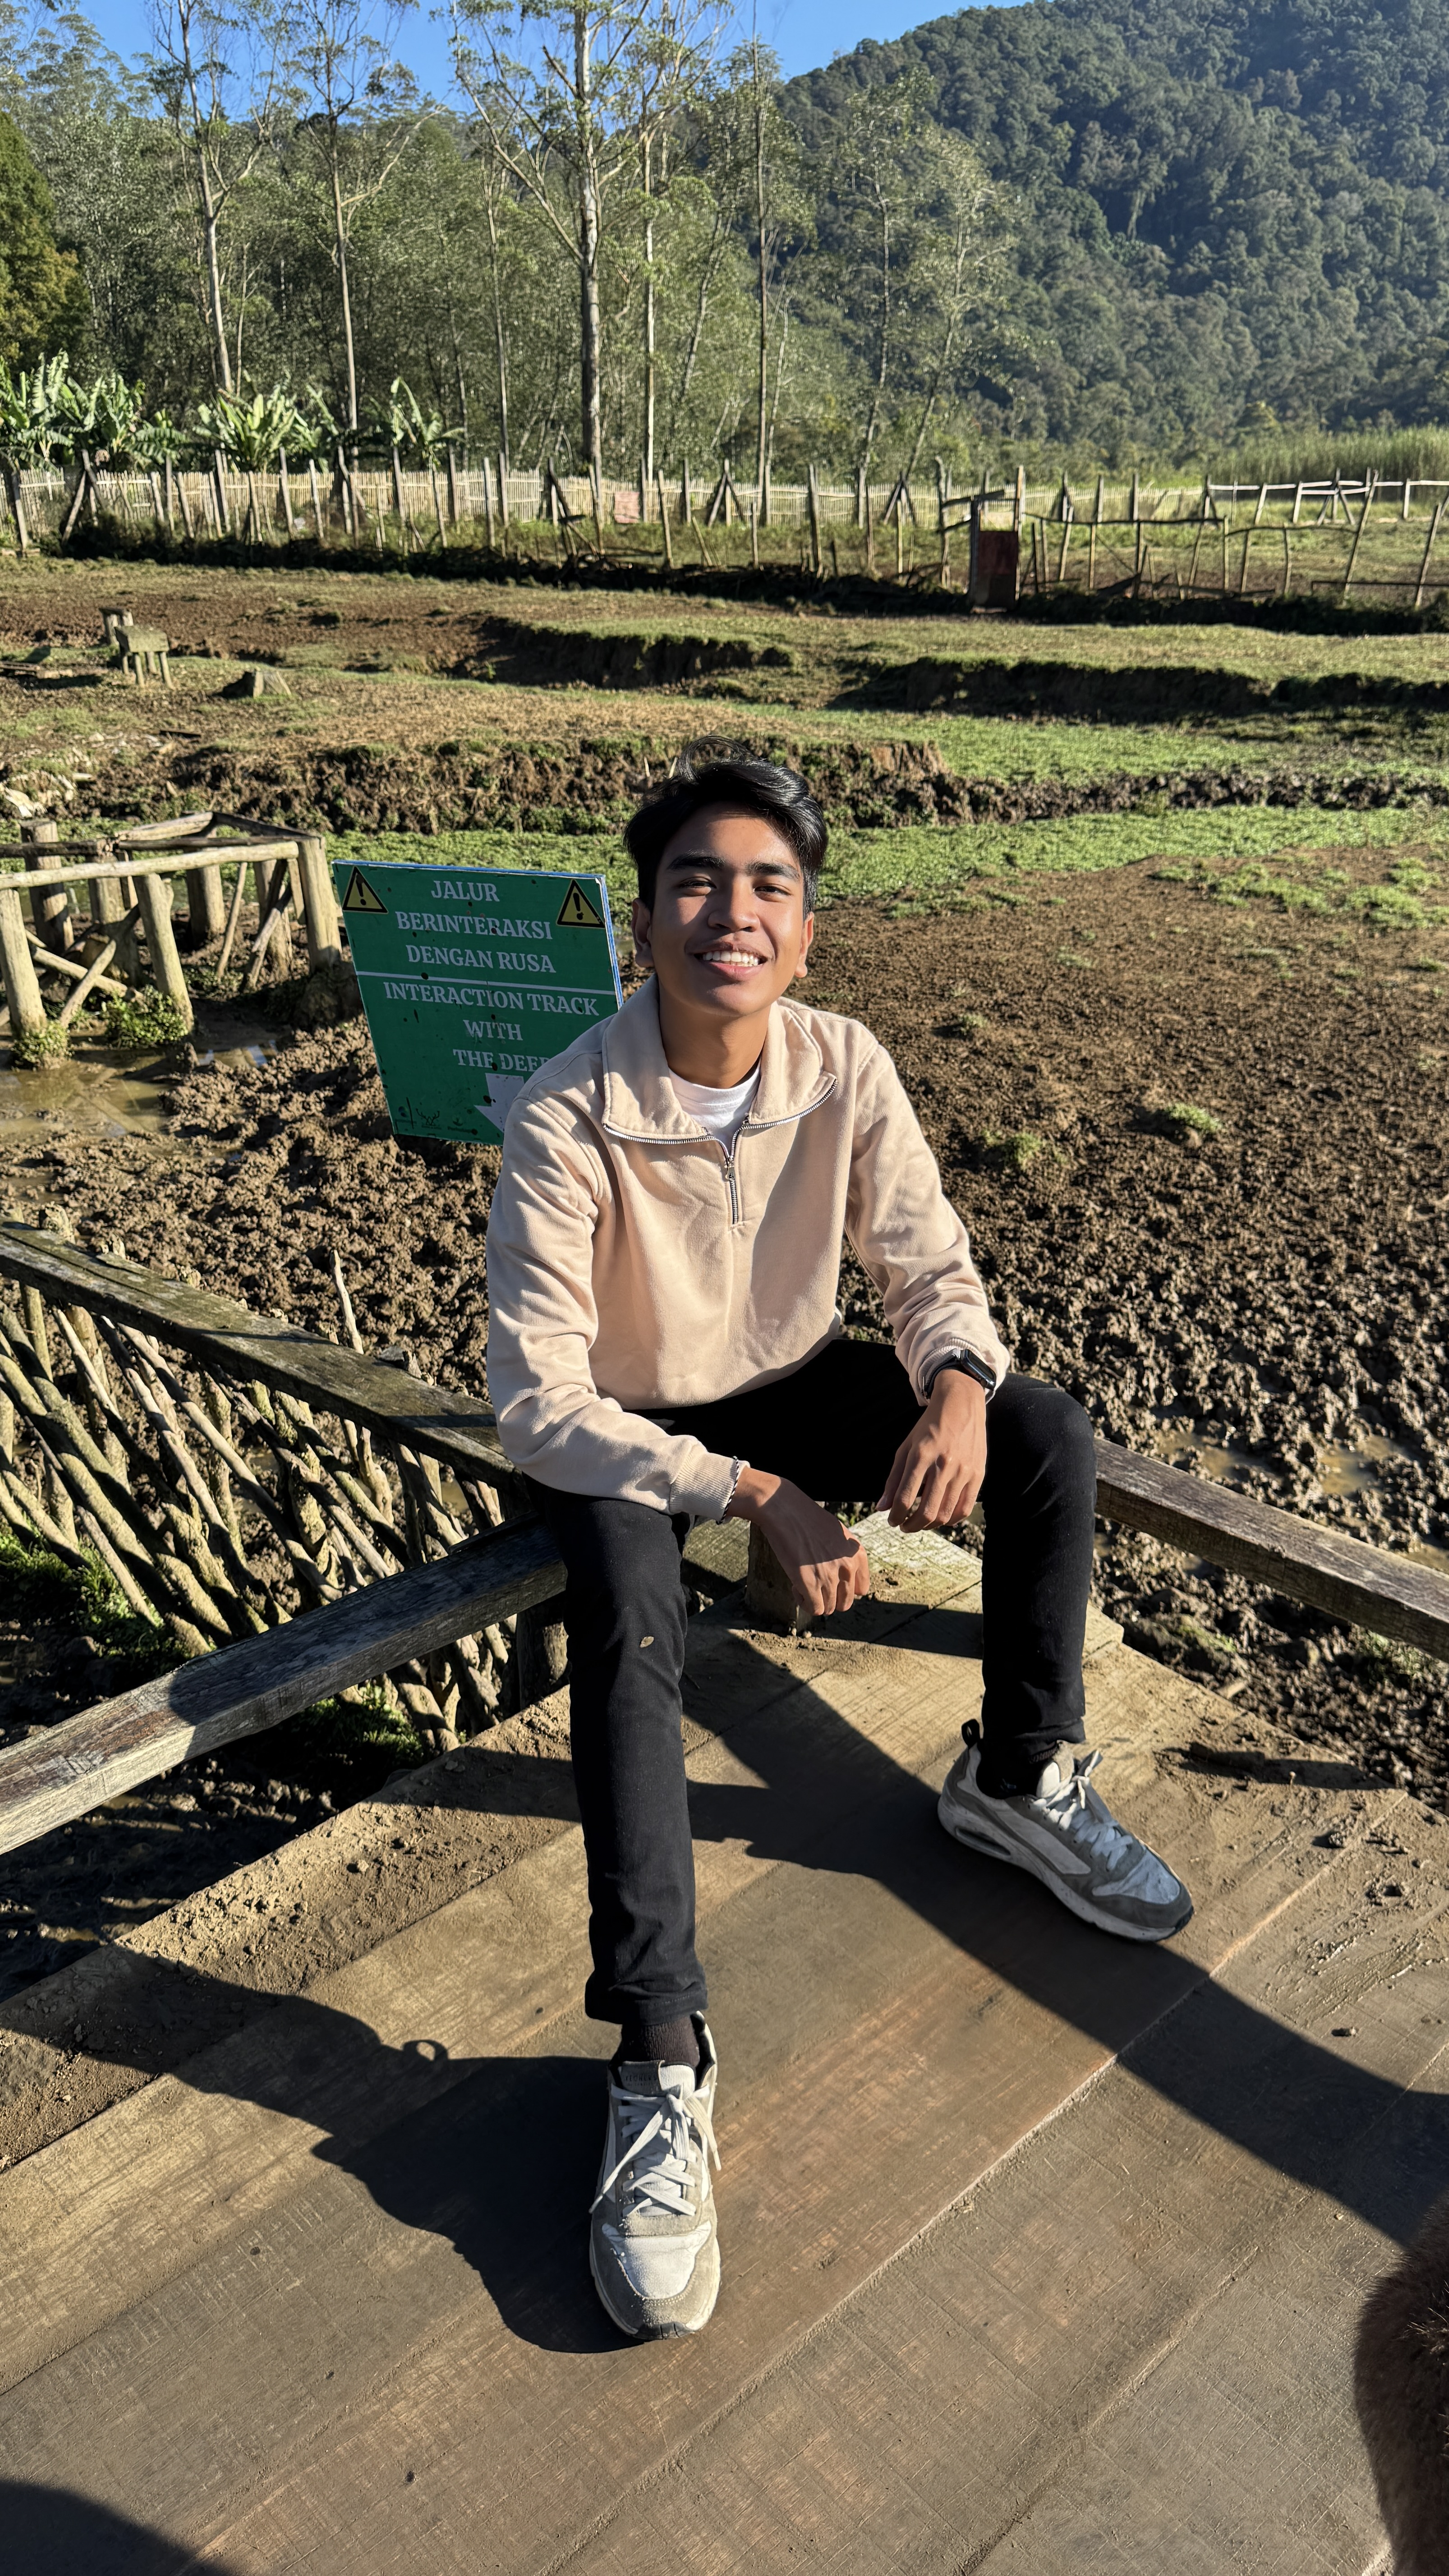
\includegraphics[width=3.125in,height=\textheight,keepaspectratio]{images/IMG_9791.JPG}

}

\caption{Foto Lukman Hakim Syah Ardhana}

\end{figure}%

Selamat datang di website ini, yang dibuat sebagai bagian dari tugas
mata kuliah \textbf{II2100 -- Komunikasi Interpersonal dan Publik} pada
Program Studi Sistem dan Teknologi Informasi, Sekolah Teknik Elektro dan
Informatika -- Institut Teknologi Bandung (ITB).

Website ini bertujuan untuk mendokumentasikan proses pembelajaran,
refleksi pribadi, serta karya-karya yang dihasilkan selama perkuliahan.
Setiap bagian dirancang untuk menunjukkan bagaimana konsep-konsep
komunikasi, seperti kesadaran diri, empati, mendengarkan aktif, hingga
komunikasi publik, dapat diterapkan dalam kehidupan akademik maupun
profesional.

Melalui pembuatan website ini, saya ingin memperlihatkan bahwa
komunikasi bukan hanya soal berbicara di depan orang banyak atau
menyampaikan informasi, tetapi juga tentang membangun makna bersama,
memahami perspektif orang lain, dan mengekspresikan diri secara jujur
dan efektif. Setiap konten yang disajikan di sini mencerminkan upaya
untuk mengaitkan teori yang dipelajari dengan pengalaman pribadi, serta
bagaimana pengalaman tersebut membentuk cara saya berkomunikasi dalam
berbagai situasi.

Selain itu, website ini juga berfungsi sebagai media refleksi, di mana
setiap karya, tulisan, maupun dokumentasi yang disertakan diharapkan
dapat memberikan pemahaman yang lebih mendalam mengenai hubungan antara
teori komunikasi dan praktik nyata. Pengunjung diajak untuk menjelajahi
setiap bagian, memahami konteks di balik karya, dan melihat bagaimana
penerapan komunikasi dapat meningkatkan kualitas interaksi, kolaborasi,
dan pemahaman antarindividu.

Dengan navigasi yang jelas dan terstruktur, pengunjung dapat dengan
mudah menjelajahi berbagai bagian website, menemukan konten yang
relevan, dan mendapatkan pengalaman belajar yang interaktif. Tujuan
akhirnya adalah agar website ini tidak hanya memenuhi persyaratan
akademik, tetapi juga menjadi contoh bagaimana komunikasi yang efektif
dapat diwujudkan melalui penyampaian informasi yang tepat, terstruktur,
dan bermakna.

\section*{Navigasi}\label{navigasi}
\addcontentsline{toc}{section}{Navigasi}

\markright{Navigasi}

\begin{itemize}
\tightlist
\item
  \href{All_About_me/index.qmd}{UTS-1 All About Me}
\item
  \href{My_Song_for_You/index.qmd}{UTS-2 My Songs for You}
\item
  \href{My_Stories_for_You/index.qmd}{UTS-3 My Stories for You}
\item
  \href{My_Shapes/index.qmd}{UTS-4 My SHAPE}
\item
  \href{My_Personal_Reviews/index.qmd}{UTS-5 My Personal Reviews}
\end{itemize}

\section*{Highlight}\label{highlight}
\addcontentsline{toc}{section}{Highlight}

\markright{Highlight}

Jelajahi berbagai karya dan refleksi yang telah disusun di bagian UTS.
Klik salah satu tautan di atas untuk melihat konten yang diinginkan,
memahami proses pembelajaran yang dilakukan, dan mendapatkan wawasan
mengenai bagaimana penerapan konsep komunikasi dapat membantu membangun
hubungan yang lebih efektif dan bermakna.

\bookmarksetup{startatroot}

\chapter{All About Me}\label{all-about-me}

\section{Awal Perjalanan}\label{awal-perjalanan}

Halo, aku Lukman. Sejak kecil, aku selalu punya rasa ingin tahu yang
besar tentang banyak hal. Aku bukan tipe anak yang gampang puas dengan
satu jawaban; kalau ada sesuatu yang bikin penasaran, aku bakal cari
tahu sampai benar-benar paham. Pernah suatu kali aku iseng membongkar
jam tangan tua bapak, cuma buat ngerti mekanismenya, akhirnya malah
copot semua gear-nya, tapi aku senang karena ngerti cara kerjanya!
Momen-momen kecil kaya gini bikin aku belajar bahwa kadang jatuh itu
bagian dari proses memahami dunia.

Aku tumbuh dengan banyak pengalaman yang pelan-pelan membentuk cara
pandangku terhadap dunia. Ada momen-momen kecil yang mungkin bagi orang
lain nggak signifikan, tapi buatku justru jadi fondasi penting---misal,
waktu aku bantu teman yang baru pindah kos, cuma dengerin dia curhat
semalam suntuk; aku sadar, kadang daya tarik seorang teman bukan soal
prestasi, tapi kemampuan kita buat hadir dan mendengar.

\section{Tentang Aku}\label{tentang-aku}

Aku orangnya reflektif dan gampang mikir hal-hal kecil. Kadang aku bisa
diem lama cuma buat merenungkan satu kejadian, satu kalimat, atau
ekspresi orang. Humor juga penting buatku---misal, aku pernah panik
karena salah kirim chat ke dosen, rasanya pengen nyebur ke kolam, tapi
sekarang aku cuma ketawa sendiri. Humor kecil seperti ini bikin
interaksi sehari-hari terasa lebih ringan, sekaligus ngebuka cara aku
berkomunikasi dengan orang lain.

Aku juga cukup perfeksionis dalam beberapa hal. Kalau ngerjain sesuatu,
aku pengen hasilnya maksimal, meskipun kadang bikin aku kelelahan. Tapi
aku sadar, hidup bukan soal kesempurnaan, tapi gimana kita bisa tetap
melangkah. Aku belajar buat lebih nerima diri sendiri, dengan segala
kekurangan dan kelebihannya---dan itu bikin cara aku berinteraksi dengan
orang lain lebih tulus, karena aku nggak terlalu takut dinilai salah.

\section{Perjalanan Akademik}\label{perjalanan-akademik}

Perjalanan akademikku nggak selalu lurus. Ada masa-masa capek, stuck,
dan ragu sama diri sendiri. Tapi ada juga momen bangga karena berhasil
melewati sesuatu yang dulu kupikir mustahil. Kuliah ngajarin aku bahwa
komunikasi itu bukan cuma soal ngomong; mendengar aktif, merespon dengan
empati, dan memahami konteks orang lain itu sama pentingnya.

Aku belajar lebih disiplin, mengatur waktu, dan nggak gampang nyerah.
Banyak hal yang awalnya bikin stres, sekarang jadi pelajaran berharga.
Misal, waktu presentasi kelompok pertama, aku sempat salah paham sama
teman tentang siapa yang bawain materi. Awalnya panik, tapi akhirnya
kami ketawa bareng sambil belajar cara koordinasi lebih efektif.
Pengalaman ini bikin aku sadar: kemampuan berkomunikasi itu bisa bikin
situasi berat jadi ringan, dan hubungan antar manusia lebih hangat.

\section{Hal-hal yang Aku Sukai}\label{hal-hal-yang-aku-sukai}

Di luar akademik, aku suka musik malam-malam, rasanya kaya ngobrol sama
diri sendiri lewat nada dan lirik. Aku juga suka nulis cerita atau
curhatan, karena itu bikin aku lebih reflektif dan sadar sama perasaan
sendiri maupun orang lain. Aku suka ngamatin orang; bukan kepo, tapi
menikmati cara setiap orang punya keunikan masing-masing. Gesture kecil,
ekspresi, atau reaksi mereka bikin aku belajar banyak soal interaksi
interpersonal.

Aku pernah ketawa sendiri liat teman kuliah yang panik karena salah baca
slide, atau waktu aku dan teman saling balas chat ngawur. Humor-humor
kecil ini bikin aku sadar: hubungan manusia itu nggak selalu serius, dan
kemampuan untuk mencairkan suasana itu bagian dari daya tarik
interpersonal yang penting.

\section{Refleksi Pribadi}\label{refleksi-pribadi}

Kalau ngeliat ke belakang, aku bersyukur sama semua proses yang udah aku
lewatin. Meski jatuh, semua itu bikin aku lebih peka, lebih kuat, dan
lebih ngerti siapa diriku. Aku belajar bahwa komunikasi itu bukan cuma
soal kata-kata, tapi juga cara kita hadir untuk orang lain. Misal,
mendengar teman curhat tanpa menilai, atau mampu menahan diri dari
reaksi impulsif, bikin hubungan lebih hangat dan tulus.

Aku masih jauh dari kata ``selesai,'' tapi aku sadar satu hal: aku jalan
bukan cuma buat nyenengin orang lain, tapi juga buat bahagiain diri
sendiri. Setiap momen lucu, gagal, atau membingungkan, adalah latihan
buat jadi versi diri yang lebih bijaksana, lebih sabar, dan lebih
empatik.

Aku percaya setiap orang punya waktunya masing-masing. Aku pelan-pelan
ngebangun hidup yang aku pengen, versi diriku sendiri. Dan yang paling
penting, aku belajar bahwa daya tarik sejati bukan cuma soal tampil
menarik, tapi kemampuan memahami, menghargai, dan hadir secara tulus
bagi orang lain.

\bookmarksetup{startatroot}

\chapter{UTS-2 My Songs for You}\label{uts-2-my-songs-for-you}

\bookmarksetup{startatroot}

\chapter{Halfway Home 🎵}\label{halfway-home}

oleh \textbf{Lukman Hakim Syah Ardhana}

\begin{center}\rule{0.5\linewidth}{0.5pt}\end{center}

\section{Tentang Karya}\label{tentang-karya}

\emph{``Halfway Home''} saya buat sebagai refleksi perjalanan pulang ---
bukan hanya pulang secara fisik, tapi juga secara emosional.\\
Lagu ini menggambarkan fase di mana seseorang belum sepenuhnya sembuh,
namun sudah cukup kuat untuk melangkah kembali ke arah yang lebih
tenang.

Karya ini selaras dengan pembelajaran di mata kuliah \textbf{Komunikasi
Interpersonal \& Publik}, di mana saya belajar bahwa proses memahami
diri sendiri dan orang lain adalah bagian dari ``pulang'' itu sendiri
--- dari konflik, dialog, hingga menerima diri.

\begin{center}\rule{0.5\linewidth}{0.5pt}\end{center}

\section{Proses Kreatif}\label{proses-kreatif}

Lagu ini saya tulis sepenuhnya berdasarkan refleksi pribadi.\\
Produksi musiknya dibuat menggunakan \textbf{Suno.ai}, sementara proses
\textbf{video editing dan visualisasi dilakukan di CapCut dan Canva}
untuk menjaga tone yang lembut dan personal.

Fokus saya bukan pada kompleksitas teknologinya, melainkan pada pesan
yang ingin disampaikan: bahwa meski belum sepenuhnya ``sampai rumah'',
perjalanan pulang itu sendiri tetap berarti.

\begin{center}\rule{0.5\linewidth}{0.5pt}\end{center}

\section{Video Karya}\label{video-karya}

\href{https://youtu.be/qKywgE79b1Q}{🎬 Tonton di YouTube}

\begin{center}\rule{0.5\linewidth}{0.5pt}\end{center}

\section{Lirik Lagu}\label{lirik-lagu}

\subsection{\texorpdfstring{\textbf{Halfway Home --- Lukman Hakim Syah
Ardhana}}{Halfway Home --- Lukman Hakim Syah Ardhana}}\label{halfway-home-lukman-hakim-syah-ardhana}

\textbf{Verse 1}\\
I walked through empty streets again\\
The lights were dim, but not the pain\\
I thought I'd heal, I thought I'd grow\\
But healing's slow --- I should've known

\textbf{Pre-Chorus}\\
The echoes call me where I've been\\
But I'm not lost, just in between

\textbf{Chorus}\\
Halfway home, I'm on my way\\
Not the end, but that's okay\\
The night still hums, the stars still show\\
I'm not there yet --- but I'll go

\textbf{Verse 2}\\
I left the ghosts where memories sleep\\
The promises I couldn't keep\\
I learned that peace is never fast\\
You find it slow, you make it last

\textbf{Pre-Chorus}\\
I still fall down, I still rewind\\
But losing's part of being kind

\textbf{Chorus}\\
Halfway home, I'm on my way\\
I'll keep walking come what may\\
The road is rough, but I still know\\
I'm halfway there --- halfway home

\textbf{Outro}\\
Maybe home's not where I've been\\
But where I choose to start again

\begin{center}\rule{0.5\linewidth}{0.5pt}\end{center}

© 2025 Lukman Hakim Syah Ardhana · Video by CapCut \& Canva ·
\href{https://youtu.be/qKywgE79b1Q}{Tonton di YouTube}

\bookmarksetup{startatroot}

\chapter{My Stories for You}\label{my-stories-for-you}

\textbf{``Jejak Waktu dan Pilihan''}\\
Ditulis oleh Lukman Hakim

Sore itu, aku duduk di tepi danau kecil dekat kampus, menatap permukaan
air yang berkilau diterpa sinar senja. Angin lembut membawa aroma
pepohonan, dan seketika kesunyian itu membuatku merenung tentang
perjalanan hidup sendiri, tentang keputusan, kehilangan, kegagalan, dan
pelajaran yang tak tertulis di buku manapun.

Aku ingat saat pertama kali menghadapi kegagalan besar, ketika segala
rencana yang kupikir matang ternyata berakhir tidak sesuai harapan.
Rasanya hampa, dan sempat terlintas ingin menyerah. Namun, perlahan aku
menyadari bahwa setiap kegagalan meninggalkan jejak, bukan untuk
membuatku terpuruk, tapi untuk mengajarkan sesuatu yang lebih berharga:
kesabaran, ketekunan, dan keberanian untuk mencoba lagi.

Di tengah perjalanan itu, aku belajar bahwa tidak semua orang yang kita
percayai akan selalu ada di sisi kita. Ada yang pergi tanpa penjelasan,
ada yang datang hanya sebentar, dan ada pula yang tetap hadir meski tak
sempurna. Aku mulai memahami bahwa cinta, persahabatan, dan hubungan
apapun bukan soal seberapa lama mereka tinggal, tapi tentang bagaimana
interaksi itu membentuk siapa kita dan apa yang kita pelajari dari
setiap pertemuan.

Malam itu, di bawah cahaya bulan yang samar, aku menulis refleksi
pertama tentang hidupku: bahwa semua yang terjadi, baik manis maupun
pahit, membentuk jalan yang kupilih sekarang. Aku belajar untuk
menerima, bukan sekadar memaafkan. Aku belajar untuk memberi ruang bagi
diri sendiri, bukan hanya bagi orang lain. Dan yang paling penting, aku
belajar bahwa kekuatan terbesar bukan datang dari mengendalikan situasi,
tapi dari memahami dan mengendalikan diri sendiri.

Hari-hari berikutnya, aku mencoba untuk lebih memperhatikan hal-hal
kecil. Sebuah senyum teman di lorong kampus, suara tawa di kelas, aroma
kopi di pagi hari, semua itu jadi pengingat bahwa hidup tak selalu soal
masalah besar. Ada keindahan yang tersembunyi di setiap momen sederhana,
dan aku belajar untuk menikmatinya tanpa harus selalu mencari makna
besar di baliknya.

Kadang aku tersenyum sendiri mengingat masa-masa ketika keputusan
sederhana terasa seperti ujian besar. Aku pernah panik memilih topik
tugas kuliah, bingung memutuskan kapan harus bicara jujur ke teman,
bahkan khawatir kalau pesan WhatsAppku dibaca salah. Semua hal kecil
itu, yang dulu terasa menegangkan, kini kurasa bagian dari latihan untuk
menjadi lebih sabar, lebih pengertian, dan lebih bijaksana. Aku
berpikir, mungkin hidup memang seperti danau yang tenang di permukaan,
tapi di bawahnya ada arus kuat yang terus bergerak, menguji kita, dan
mengingatkan kita untuk tetap berhati-hati tapi berani melangkah.

Suatu malam, aku menulis catatan panjang di buku harian. Aku mencatat
kegagalan, rasa takut, dan harapan. Aku menulis momen-momen ketika aku
merasa kurang berdaya, ketika aku hampir menyerah, dan ketika aku
berhasil menahan diri dari keputusan impulsif. Aku menulis juga tentang
hal-hal lucu yang terjadi sehari-hari, seperti tumpukan buku yang hampir
jatuh, atau chat yang salah kirim, karena aku sadar bahwa belajar dari
hidup tak selalu serius; kadang humor kecil membuat kita kuat.

Aku menulis tentang hubungan-hubungan yang pernah aku jalani, tentang
bagaimana aku belajar memberi batas, menerima perbedaan, dan memahami
bahwa orang lain juga punya perjalanan sendiri. Aku belajar bahwa
mencintai orang lain harus dimulai dari mencintai diri sendiri. Jangan
sampai hati kita habis hanya karena menunggu pengakuan yang tak pernah
datang.

Aku juga menulis tentang mimpi dan ambisi, tentang bagaimana kadang rasa
takut gagal membuat langkah terhenti, tapi jika tidak mencoba, kita
tidak akan pernah tahu batas kemampuan diri sendiri. Aku menuliskan rasa
malu, rasa kecewa, dan rasa bangga pada diri sendiri yang masih mencoba
walau sering gagal. Semua itu menjadi pelajaran berharga yang membentuk
karakterku hari ini.

Di malam yang tenang, aku menatap danau lagi, membayangkan masa depan
dan tersenyum pada diri sendiri. Tersenyum karena aku telah melewati
banyak hal, belajar dari kesalahan, dan masih mampu percaya pada diri
sendiri. Aku menulis bahwa perjalanan hidup ini seperti buku yang tak
pernah berhenti dicetak: setiap halaman punya cerita, dan setiap cerita
punya makna tersendiri.

Sekarang, aku menulis bukan hanya untuk mengingat masa lalu, tapi untuk
merayakan proses menjadi diri sendiri. Setiap cerita, setiap kegagalan,
dan setiap keberhasilan adalah jejak waktu yang membentukku. Aku sadar,
tidak ada yang instan, semua butuh waktu, kesabaran, dan refleksi. Dan
di setiap langkah yang kuambil, aku berjanji pada diri sendiri untuk
terus belajar, terus bertumbuh, dan terus menghargai perjalanan ini,
seberat apapun ombak yang menghadang.

Suatu hari nanti, aku berharap bisa membagikan pengalaman ini ke orang
lain, agar mereka juga tahu bahwa setiap jatuh dan bangkit adalah bagian
dari proses menjadi lebih bijaksana. Bahwa hidup kadang lucu, kadang
menyakitkan, tapi selalu berharga. Dan yang terpenting, setiap orang
punya kesempatan menulis cerita mereka sendiri, dengan kebijaksanaan,
kesabaran, dan hati yang terbuka.

\bookmarksetup{startatroot}

\chapter{My SHAPE}\label{my-shape}

\section{Piagam Diri (Personal
Charter)}\label{piagam-diri-personal-charter}

\begin{longtable}[]{@{}
  >{\raggedright\arraybackslash}p{(\linewidth - 2\tabcolsep) * \real{0.4286}}
  >{\raggedright\arraybackslash}p{(\linewidth - 2\tabcolsep) * \real{0.5714}}@{}}
\toprule\noalign{}
\begin{minipage}[b]{\linewidth}\raggedright
DIMENSI
\end{minipage} & \begin{minipage}[b]{\linewidth}\raggedright
PENJELASAN
\end{minipage} \\
\midrule\noalign{}
\endhead
\bottomrule\noalign{}
\endlastfoot
\textbf{S --- Signature Strengths (Kekuatan Utama)} & 1. Mampu berpikir
kritis dan jernih di tengah tekanan, melihat gambaran besar tanpa
kehilangan fokus pada detail yang penting.2. Konsisten dan gigih dalam
menyelesaikan sesuatu yang dirasa bermanfaat, meskipun butuh waktu dan
usaha ekstra.3. Fleksibel dan terbuka pada ide baru, serta mampu
beradaptasi dengan orang dari berbagai latar belakang. \\
\textbf{H --- Heart (Nilai dan Hal yang Diperjuangkan)} & 1. Percaya
bahwa ilmu dan teknologi harus digunakan untuk memberi dampak positif
bagi banyak orang, bukan sekadar prestasi pribadi.2. Menjunjung tinggi
integritas, empati, dan kerja sama sebagai fondasi interaksi
sehari-hari.3. Merasa paling hidup ketika bisa membantu orang lain,
membimbing, atau berkontribusi dalam proyek yang memberi manfaat
nyata. \\
\textbf{A --- Aptitudes \& Acquired Skills (Kemampuan dan Keterampilan)}
& 1. Terbiasa menganalisis pola, memahami masalah dengan cara logis,
serta membuat keputusan berbasis data dan pertimbangan matang.2.
Terampil bekerja dalam tim, membagi peran, dan mengatur waktu agar hasil
tetap berkualitas dan tepat waktu.3. Mampu menjelaskan ide atau konsep
kompleks dengan bahasa yang mudah dipahami, baik lewat tulisan maupun
percakapan. \\
\textbf{P --- Personality (Kepribadian)} & Tenang, reflektif, dan
berhati-hati dalam bertindak. Lebih memilih makna daripada rutinitas
kosong, serta berperan sebagai pendengar yang baik dan mediator dalam
tim. \\
\textbf{E --- Experiences (Pengalaman Hidup)} & 1. Mengikuti proyek dan
kompetisi yang mempertemukan orang dari berbagai latar belakang,
sehingga belajar pentingnya komunikasi terbuka dan saling menghargai.2.
Mengalami langsung bagaimana ketekunan, empati, dan kerja sama
menentukan keberhasilan di lingkungan akademik maupun profesional.3.
Menyadari bahwa setiap pengalaman, baik tantangan maupun keberhasilan,
memberikan pelajaran baru tentang diri sendiri dan kemampuan
berinteraksi. \\
\end{longtable}

\section{Pernyataan Misi Pribadi}\label{pernyataan-misi-pribadi}

Saya berkomitmen untuk menghubungkan pengetahuan, kemampuan, dan
manusia: memanfaatkan apa yang saya pelajari untuk memberi dampak
positif, membantu orang tumbuh, dan memperkuat hubungan yang tulus dan
saling menghargai. Saya ingin setiap karya, kolaborasi, dan interaksi
saya tidak hanya memberi manfaat nyata bagi orang lain, tapi juga
menumbuhkan kesadaran diri dan empati di lingkungan sekitar.

Saya percaya bahwa kekuatan diri bukan hanya soal skill atau prestasi,
tapi juga kemampuan untuk hadir, mendengar, dan memberi dampak positif
lewat tindakan nyata. Setiap langkah, keputusan, dan interaksi harus
konsisten dengan prinsip integritas, empati, dan kontribusi yang
bermakna.

\bookmarksetup{startatroot}

\chapter{UTS-5 My Personal Reviews}\label{uts-5-my-personal-reviews}

\section{Identifikasi}\label{identifikasi}

\begin{longtable}[]{@{}ll@{}}
\toprule\noalign{}
Nama & NIM \\
\midrule\noalign{}
\endhead
\bottomrule\noalign{}
\endlastfoot
\textbf{Lukman Hakim Syah Ardhana} & \textbf{18224097} \\
\end{longtable}

\begin{center}\rule{0.5\linewidth}{0.5pt}\end{center}

\section{Tinjauan Umum}\label{tinjauan-umum}

Karya web \textbf{All About Me} karya Lukman menampilkan kepribadian
reflektif, orisinal, dan ekspresif. Setiap bagian UTS (1--5) menunjukkan
perkembangan naratif dan kedewasaan komunikasi personal. Secara umum,
seluruh konten konsisten dengan tema kuliah \emph{Komunikasi
Interpersonal} --- menggambarkan kesadaran diri, empati, dan gaya pesan
yang autentik.

\begin{center}\rule{0.5\linewidth}{0.5pt}\end{center}

\section{Tinjauan Spesifik}\label{tinjauan-spesifik}

\subsection{UTS-1: All About Me}\label{uts-1-all-about-me}

Narasi reflektif tentang perjalanan pribadi yang penuh keingintahuan dan
kejujuran diri.

\begin{longtable}[]{@{}
  >{\raggedright\arraybackslash}p{(\linewidth - 6\tabcolsep) * \real{0.2973}}
  >{\raggedright\arraybackslash}p{(\linewidth - 6\tabcolsep) * \real{0.3243}}
  >{\raggedright\arraybackslash}p{(\linewidth - 6\tabcolsep) * \real{0.1622}}
  >{\raggedright\arraybackslash}p{(\linewidth - 6\tabcolsep) * \real{0.2162}}@{}}
\toprule\noalign{}
\begin{minipage}[b]{\linewidth}\raggedright
Kriteria
\end{minipage} & \begin{minipage}[b]{\linewidth}\raggedright
Deskripsi
\end{minipage} & \begin{minipage}[b]{\linewidth}\raggedright
Skor
\end{minipage} & \begin{minipage}[b]{\linewidth}\raggedright
Level
\end{minipage} \\
\midrule\noalign{}
\endhead
\bottomrule\noalign{}
\endlastfoot
\textbf{Orisinalitas} & Menampilkan kisah diri yang unik dan otentik
tanpa klise. & 5 & Sangat Baik \\
\textbf{Keterlibatan} & Cerita mengalir dan menjaga perhatian pembaca. &
4 & Baik \\
\textbf{Humor} & Ada sedikit kehangatan natural, meski bukan fokus
utama. & 3 & Cukup \\
\textbf{Wawasan (Insight)} & Menunjukkan pemahaman diri dan refleksi
mendalam. & 5 & Sangat Baik \\
\end{longtable}

\textbf{Komentar \& Saran:}\\
Tulisan ini jujur dan mengalir alami. Bisa ditingkatkan dengan
menambahkan sedikit variasi emosional atau anekdot ringan agar lebih
hidup.

\begin{center}\rule{0.5\linewidth}{0.5pt}\end{center}

\subsection{UTS-2: Songs for You (``Halfway Home
🎵'')}\label{uts-2-songs-for-you-halfway-home}

Puisi reflektif yang puitis dan berkesan, dengan makna pulang secara
emosional dan spiritual.

\begin{longtable}[]{@{}
  >{\raggedright\arraybackslash}p{(\linewidth - 6\tabcolsep) * \real{0.2973}}
  >{\raggedright\arraybackslash}p{(\linewidth - 6\tabcolsep) * \real{0.3243}}
  >{\raggedright\arraybackslash}p{(\linewidth - 6\tabcolsep) * \real{0.1622}}
  >{\raggedright\arraybackslash}p{(\linewidth - 6\tabcolsep) * \real{0.2162}}@{}}
\toprule\noalign{}
\begin{minipage}[b]{\linewidth}\raggedright
Kriteria
\end{minipage} & \begin{minipage}[b]{\linewidth}\raggedright
Deskripsi
\end{minipage} & \begin{minipage}[b]{\linewidth}\raggedright
Skor
\end{minipage} & \begin{minipage}[b]{\linewidth}\raggedright
Level
\end{minipage} \\
\midrule\noalign{}
\endhead
\bottomrule\noalign{}
\endlastfoot
\textbf{Orisinalitas} & Tema perjalanan batin digarap segar dan
simbolis. & 5 & Sangat Baik \\
\textbf{Keterlibatan} & Lirik mampu mengundang imajinasi dan empati. & 4
& Baik \\
\textbf{Humor} & Tidak dominan, namun terasa ringan di beberapa frasa. &
3 & Cukup \\
\textbf{Inspirasi} & Menghadirkan makna pulang dengan pesan universal. &
5 & Sangat Baik \\
\end{longtable}

\textbf{Komentar \& Saran:}\\
Pilihan diksi sangat kuat. Untuk pengembangan, bisa tambahkan konteks
visual atau audio agar pengalaman lebih imersif.

\begin{center}\rule{0.5\linewidth}{0.5pt}\end{center}

\subsection{UTS-3: My Stories for You (``Jejak Waktu dan
Pilihan'')}\label{uts-3-my-stories-for-you-jejak-waktu-dan-pilihan}

Cerita pendek dengan narasi introspektif dan nilai moral yang jelas.

\begin{longtable}[]{@{}
  >{\raggedright\arraybackslash}p{(\linewidth - 6\tabcolsep) * \real{0.2973}}
  >{\raggedright\arraybackslash}p{(\linewidth - 6\tabcolsep) * \real{0.3243}}
  >{\raggedright\arraybackslash}p{(\linewidth - 6\tabcolsep) * \real{0.1622}}
  >{\raggedright\arraybackslash}p{(\linewidth - 6\tabcolsep) * \real{0.2162}}@{}}
\toprule\noalign{}
\begin{minipage}[b]{\linewidth}\raggedright
Kriteria
\end{minipage} & \begin{minipage}[b]{\linewidth}\raggedright
Deskripsi
\end{minipage} & \begin{minipage}[b]{\linewidth}\raggedright
Skor
\end{minipage} & \begin{minipage}[b]{\linewidth}\raggedright
Level
\end{minipage} \\
\midrule\noalign{}
\endhead
\bottomrule\noalign{}
\endlastfoot
\textbf{Orisinalitas} & Tema waktu dan pilihan disajikan segar dan
personal. & 4 & Baik \\
\textbf{Keterlibatan} & Cerita membangun emosi dengan ritme yang halus.
& 4 & Baik \\
\textbf{Pengembangan Narasi} & Struktur cerita rapi dengan kesinambungan
logis. & 4 & Baik \\
\textbf{Inspirasi} & Mengandung refleksi hidup yang relevan dan positif.
& 5 & Sangat Baik \\
\end{longtable}

\textbf{Komentar \& Saran:}\\
Ceritanya efektif menyentuh sisi reflektif pembaca. Akan lebih kuat bila
menambahkan konflik kecil untuk memperdalam pesan.

\begin{center}\rule{0.5\linewidth}{0.5pt}\end{center}

\subsection{UTS-4: My SHAPE}\label{uts-4-my-shape}

Analisis diri menggunakan model SHAPE yang disajikan dalam bentuk tabel
informatif dan jujur.

\begin{longtable}[]{@{}
  >{\raggedright\arraybackslash}p{(\linewidth - 6\tabcolsep) * \real{0.2973}}
  >{\raggedright\arraybackslash}p{(\linewidth - 6\tabcolsep) * \real{0.3243}}
  >{\raggedright\arraybackslash}p{(\linewidth - 6\tabcolsep) * \real{0.1622}}
  >{\raggedright\arraybackslash}p{(\linewidth - 6\tabcolsep) * \real{0.2162}}@{}}
\toprule\noalign{}
\begin{minipage}[b]{\linewidth}\raggedright
Kriteria
\end{minipage} & \begin{minipage}[b]{\linewidth}\raggedright
Deskripsi
\end{minipage} & \begin{minipage}[b]{\linewidth}\raggedright
Skor
\end{minipage} & \begin{minipage}[b]{\linewidth}\raggedright
Level
\end{minipage} \\
\midrule\noalign{}
\endhead
\bottomrule\noalign{}
\endlastfoot
\textbf{Orisinalitas} & Penyusunan tabel SHAPE unik dan menunjukkan
pemahaman diri. & 4 & Baik \\
\textbf{Keterlibatan} & Menarik karena penyajian visual dan sistematis.
& 4 & Baik \\
\textbf{Pengembangan Narasi} & Penjelasan tiap aspek (Strength, Heart,
Ability, Personality, Experience) jelas. & 5 & Sangat Baik \\
\textbf{Inspirasi} & Menginspirasi pembaca untuk mengenali potensi diri.
& 5 & Sangat Baik \\
\end{longtable}

\textbf{Komentar \& Saran:}\\
Sudah sangat terstruktur. Bisa lebih kuat jika disertai contoh konkret
pengalaman untuk tiap dimensi SHAPE.

\begin{center}\rule{0.5\linewidth}{0.5pt}\end{center}

\subsection{UTS-5: My Personal Review}\label{uts-5-my-personal-review}

Review reflektif menggunakan bantuan ChatGPT untuk menilai karya
sendiri; menunjukkan kesadaran metakognitif tinggi.

\begin{longtable}[]{@{}
  >{\raggedright\arraybackslash}p{(\linewidth - 6\tabcolsep) * \real{0.2973}}
  >{\raggedright\arraybackslash}p{(\linewidth - 6\tabcolsep) * \real{0.3243}}
  >{\raggedright\arraybackslash}p{(\linewidth - 6\tabcolsep) * \real{0.1622}}
  >{\raggedright\arraybackslash}p{(\linewidth - 6\tabcolsep) * \real{0.2162}}@{}}
\toprule\noalign{}
\begin{minipage}[b]{\linewidth}\raggedright
Kriteria
\end{minipage} & \begin{minipage}[b]{\linewidth}\raggedright
Deskripsi
\end{minipage} & \begin{minipage}[b]{\linewidth}\raggedright
Skor
\end{minipage} & \begin{minipage}[b]{\linewidth}\raggedright
Level
\end{minipage} \\
\midrule\noalign{}
\endhead
\bottomrule\noalign{}
\endlastfoot
\textbf{Pemahaman Konsep Interpersonal} & Menunjukkan pemahaman kuat
tentang komunikasi diri dan evaluasi personal. & 5 & Sangat Baik \\
\textbf{Analisis Kritis Pesan} & Menilai dengan kritis dan seimbang
antara kekuatan dan kelemahan. & 4 & Baik \\
\textbf{Argumentasi (Logos)} & Logis dan disusun sistematis. & 4 &
Baik \\
\textbf{Etos \& Empati} & Menunjukkan empati terhadap diri dan proses
belajar. & 5 & Sangat Baik \\
\textbf{Rekomendasi Perbaikan} & Memberikan refleksi perbaikan yang
aplikatif. & 5 & Sangat Baik \\
\end{longtable}

\textbf{Komentar \& Saran:}\\
Pendekatan reflektif berbasis AI ini menarik dan inovatif. Bisa lebih
kuat bila dikaitkan eksplisit dengan teori komunikasi interpersonal dari
perkuliahan.

\begin{center}\rule{0.5\linewidth}{0.5pt}\end{center}

\section{Rekap Skor dan Kontribusi
CPMK}\label{rekap-skor-dan-kontribusi-cpmk}

\begin{longtable}[]{@{}llll@{}}
\toprule\noalign{}
UTS & Rata-rata Skor (1--5) & Persentase & CPMK Terkait \\
\midrule\noalign{}
\endhead
\bottomrule\noalign{}
\endlastfoot
\textbf{UTS-1 All About Me} & 4.25 & 85\% & CPMK 1, 2 \\
\textbf{UTS-2 Songs for You} & 4.25 & 85\% & CPMK 1, 2 \\
\textbf{UTS-3 My Stories for You} & 4.25 & 85\% & CPMK 1, 2 \\
\textbf{UTS-4 My SHAPE} & 4.5 & 90\% & CPMK 3 \\
\textbf{UTS-5 My Personal Review} & 4.6 & 92\% & CPMK 4 \\
\end{longtable}

\textbf{Total rerata keseluruhan: 87.4\%}

\begin{center}\rule{0.5\linewidth}{0.5pt}\end{center}

\section{Kesimpulan}\label{kesimpulan}

Lukman menunjukkan kemampuan komunikasi personal yang matang, empatik,
dan reflektif. Progres antar-UTS terasa konsisten --- dari pengenalan
diri hingga evaluasi pribadi --- semuanya mencerminkan pemahaman konsep
komunikasi interpersonal secara menyeluruh.\\
Karya ini sudah layak dinilai \textbf{Sangat Baik}, dengan potensi
penguatan pada dimensi naratif dan elaborasi teoritis untuk tahap
selanjutnya.

\bookmarksetup{startatroot}

\chapter{UAS-1 My Concepts}\label{uas-1-my-concepts}

Mau hidup epik ? \href{lifestory.pdf}{Write your Life Story}

Apa itu berkonsep?

\url{https://youtu.be/QVfUlVBO80U?si=yM6q_rwV9rcDBbu7}

\bookmarksetup{startatroot}

\chapter{UAS-3 My Opinions}\label{uas-3-my-opinions}

SApa itu beropini? \href{BM\%20Opini.mp4}{Opini Berpengaruh}

Bagiamana menjaadi menarik? \href{./Interesting.mp4}{Menjadi Menarik}

\bookmarksetup{startatroot}

\chapter{UAS-3 My Innovations}\label{uas-3-my-innovations}

\bookmarksetup{startatroot}

\chapter{UAS-4 My Knowledge}\label{uas-4-my-knowledge}

Cara saya mengkomunikasikan sebuah pengatahuan sebagai petunjuk bagi
orang lain 1) saya tulis
\href{Rekomendasi\%20Presentasi\%20Efektif(Contoh\%20Makalah).pdf}{makalah
sebagai bahan utama} 2) lalu saya buat
\href{Contoh\%20Transkrip\%20Presentasi.pdf}{transkrip ucapan lisan} 3)
kemudian saya kembangkan
\href{Rekomendasi\%20Presentasi\%20(Contoh\%20Slides).pdf}{slide
pendukung trnsskrip} 4) lalu saya memproduksivideo audio visual
\url{https://youtu.be/ZbghfMvnPZc} \url{https://youtu.be/ZbghfMvnPZc}

\bookmarksetup{startatroot}

\chapter{UAS-5 My Professional
Reviews}\label{uas-5-my-professional-reviews}

Untuk melAkukan review, seperti pada
\href{../My_Personal_Reviews/Doc.5.Mengevaluasi-Esai-Berdasarkan-Rubrik.pdf}{pendekatan
AI}, kita membutuhkan rubrik

\bookmarksetup{startatroot}

\chapter{Summary}\label{summary}

In summary, this book has no content whatsoever.

\bookmarksetup{startatroot}

\chapter*{References}\label{references}
\addcontentsline{toc}{chapter}{References}

\markboth{References}{References}

\phantomsection\label{refs}




\end{document}
